\documentclass[11pt]{article}
\usepackage{fullpage}
\usepackage{graphicx}
\usepackage{amsfonts}
\usepackage{procedure,proceduric}
%\usepackage{ipe}

\setlength{\parskip}{2ex}
 
%\usepackage{amsthm}

\newcommand{\centeripe}[1]{\begin{center}\Ipe{#1}\end{center}}
\newcommand{\comment}[1]{}

\newcommand{\centerpsfig}[1]{\centerline{\psfig{#1}}}

\newcommand{\seclabel}[1]{\label{sec:#1}}
\newcommand{\Secref}[1]{Section~\ref{sec:#1}}
\newcommand{\secref}[1]{\mbox{Section~\ref{sec:#1}}}

\newcommand{\alglabel}[1]{\label{alg:#1}}
\newcommand{\Algref}[1]{Algorithm~\ref{alg:#1}}
\newcommand{\algref}[1]{\mbox{Algorithm~\ref{alg:#1}}}

\newcommand{\applabel}[1]{\label{app:#1}}
\newcommand{\Appref}[1]{Appendix~\ref{app:#1}}
\newcommand{\appref}[1]{\mbox{Appendix~\ref{app:#1}}}

\newcommand{\tablabel}[1]{\label{tab:#1}}
\newcommand{\Tabref}[1]{Table~\ref{tab:#1}}
\newcommand{\tabref}[1]{Table~\ref{tab:#1}}

\newcommand{\figlabel}[1]{\label{fig:#1}}
\newcommand{\Figref}[1]{Figure~\ref{fig:#1}}
\newcommand{\figref}[1]{\mbox{Figure~\ref{fig:#1}}}

\newcommand{\eqlabel}[1]{\label{eq:#1}}
\newcommand{\eqref}[1]{(\ref{eq:#1})}

\newtheorem{thm}{Theorem}{\bfseries}{\itshape}
\newcommand{\thmlabel}[1]{\label{thm:#1}}
\newcommand{\thmref}[1]{Theorem~\ref{thm:#1}}

\newtheorem{lem}{Lemma}{\bfseries}{\itshape}
\newcommand{\lemlabel}[1]{\label{lem:#1}}
\newcommand{\lemref}[1]{Lemma~\ref{lem:#1}}

\newtheorem{cor}{Corollary}{\bfseries}{\itshape}
\newcommand{\corlabel}[1]{\label{cor:#1}}
\newcommand{\corref}[1]{Corollary~\ref{cor:#1}}

\newtheorem{obs}{Observation}{\bfseries}{\itshape}
\newcommand{\obslabel}[1]{\label{obs:#1}}
\newcommand{\obsref}[1]{Observation~\ref{obs:#1}}

\newtheorem{assumption}{Assumption}{\bfseries}{\rm}
\newenvironment{ass}{\begin{assumption}\rm}{\end{assumption}}
\newcommand{\asslabel}[1]{\label{ass:#1}}
\newcommand{\assref}[1]{Assumption~\ref{ass:#1}}

\newcommand{\proclabel}[1]{\label{alg:#1}}
\newcommand{\procref}[1]{Procedure~\ref{alg:#1}}

\newtheorem{rem}{Remark}
\newtheorem{op}{Open Problem}

\newcommand{\etal}{\emph{et al}}

\newcommand{\voronoi}{Vorono\u\i}
\newcommand{\ceil}[1]{\left\lceil #1 \right\rceil}
\newcommand{\floor}[1]{\left\lfloor #1 \right\rfloor}



% Use 1.3 times the normal baseline-to-baseline skip
\renewcommand{\baselinestretch}{1.3}


\title{Testing the Quality of
	Manufactured Disks and Balls%
	\thanks{This work was funded in part by the Natural
	Sciences and Engineering Research Council of Canada}}

\author{Prosenjit Bose and Pat Morin \\ School of Computer Science, 
	Carleton University, Ottawa, CANADA, K1S~5B6 \\
	\texttt{\{morin,jit\}@cs.carleton.ca}} 

\date{}

\newcommand{\mysqrt}[1]{\left({#1}\right)^\frac{1}{2}}

\newcommand{\sa}{\mathrm{sa}}
\newcommand{\origin}{o_+}

\newcommand{\bd}{\mathrm{bd}}
\newcommand{\dist}{\mathrm{dist}}
\newcommand{\probe}{\mathrm{probe}}
\newcommand{\qual}{\mathrm{qual}}
\newcommand{\x}{\mathrm{x}}
\newcommand{\y}{\mathrm{y}}
\newcommand{\z}{\mathrm{z}}
\newcommand{\jout}{J_{\mathrm{out}}}
\newcommand{\jin}{J_{\mathrm{in}}}
\newcommand{\yp}{\mathrm{y'}}
\newcommand{\ypp}{\mathrm{y''}}

%\renewcommand{\centeripe}[1]{\vspace{1cm}}
%\renewcommand{\centeripe}[1]{\begin{center}\includegraphics{#1}\end{center}}
%\newcommand{\centeripetwo}[1]{\begin{center}\Ipe{#1}\end{center}}

% The function f(n)
%\newcommand{\fn}{\frac{1}{n}\left(\frac{1+\delta}{\alpha}\right)\left(\alpha^2+1+2\delta+\delta^2\right)^\frac{1}{2}}
\newcommand{\fn}{\sqrt{\left(\frac{(1+\delta)\pi}{n}\right)^2
	+\left(\frac{(1+\delta)^2\pi}{\alpha n}\right)^2}}

\newcommand{\no}{\left\lceil\pi/\arctan(\alpha/(1+\delta))\right\rceil}

% The function g(n)
%\newcommand{\fpn}{\frac{1}{n}\left((1 + 3\delta)^2\pi^2 + \frac{(1 + 3\delta)^4\pi^2}{(\alpha - 2\delta)^2}\right)^\frac{1}{2}}
\newcommand{\fpn}{\sqrt{\left(\frac{\pi(1+3\delta)}{n}\right)^2 +
	\left(\frac{\pi(1+3\delta)^2}{n(\alpha-2\delta)}\right)^2}}


\newcommand{\npo}{\left\lceil\pi/\arctan(\alpha/(1+3\delta))\right\rceil}
 
% The function h(n)
\newcommand{\fppn}{g(n) + \frac{1}{n}\left( ((1+3\delta)\pi/\alpha)^2 + \pi^2 
                \right)^\frac{1}{2}}

\begin{document}
\maketitle

\begin{abstract}
We consider the problem of testing the roundness of manufactured disks
and balls using the finger probing model of Cole and Yap \cite{cy87}.
The running time of our procedures depends on the \emph{quality} of
the object being considered.  Quality is a parameter that is negative
when the object is not sufficiently round and positive when it is.
Quality values close to 0 represent objects that are close to the
boundary between sufficiently round and insufficiently round.

When the object being tested is a disk and its center is known, we
describe a procedure that uses $O(n)$ probes and $O(n)$ computation
time. (Here $n=|1/q|$, where $q$ is the quality of the object.)  When
the center of the object is not known, a procedure using $O(n)$ probes
and $O(n\log n)$ computation time is described.  When the object is a
ball, we describe a procedure that requires $O(n^2)$ probes and
$O(n^4)$ computation time.  Lower bounds are also given that show
that these procedures are optimal in terms of the number of probes
used.  These results extend previous results in two directions by
relaxing some of the assumptions required by previous results and by
extending these results for 3-dimensional objects.
\end{abstract}

%%%%%%%%%%%%%%%%%%%%%%%%%%%%%%%%%%%%%%%%%%%%%%%%%%%%%%%%%%%%%%%%%%%%%%%%%%
\section{Introduction}

The field of metrology is concerned with measuring the quality of
manufactured objects.  A basic task in metrology is that of
determining whether a given manufactured object is of acceptable
quality.  Usually this involves probing the surface of the object
using a measuring device such as a coordinate measuring machine to get
a set $S$ of sample points, and then verifying, algorithmically, how
well $S$ approximates an ideal object.

A special case of this problem is determining whether an object is
\emph{round}.  For our purposes, an object $I$ is \emph{good} if the
boundary of $I$ can be contained in an annulus of inner radius
$1-\epsilon$ and outer radius $1+\epsilon$, for some quality parameter
$\epsilon > 0$, and is \emph{bad} otherwise.  See \figref{first} for
examples of good and bad objects.  We call this problem the {\em
roundness classification problem.}

\begin{figure}
\begin{center}\begin{tabular}{ccc}
\includegraphics{good} & \raisebox{-1mm}{\includegraphics{bad-a}} &
\includegraphics{bad-b}
\end{tabular}\end{center}
\caption{Examples of (a) good and (b) \& (c) bad objects.  
	The inner circle has radius
	$1-\epsilon$ and the outer circle has radius $1+\epsilon$.}
\figlabel{first}
\end{figure}

In the field of computational geometry a lot of work has been done on
finding efficient algorithms for testing the roundness of a set of
sample points, using the definition of roundness given above
\cite{bbbrw98,dgr97,r97}, as well as several other definitions of
roundness
\cite{aas99,aas01,aass99,c00,efnn92,gr98,ks99,ll91,rz92,r99,ssty96,s93}.

However, very little research has been done on probing strategies for
the roundness classification problem.  A notable exception is the work
by \mbox{Mehlhorn}, \mbox{Shermer}, and \mbox{Yap} \cite{msy97,sy95},
in which a probing strategy for manufactured disks is coupled with a
roundness testing algorithm.  Unfortunately, the procedure described
in \cite{msy97,sy95} relies on the assumption that the object $I$ is
convex. It is usually not the case that the manufacturing process can
guarantee this.

In this paper we describe strategies for testing the roundness of
manufactured disks and balls.  We use the \emph{finger probing} model
of \mbox{Cole} and \mbox{Yap} \cite{cy87}.  In this model, the
measurement device can identify a point in the interior of $I$ and can
probe along any ray originating outside of $I$, i.e., determine the
first point on the ray that intersects the boundary of $I$ (see
\figref{cmm}). The finger probing model is a reasonable abstract model
of a coordinate measuring machine or a laser range-finder \cite{y94}.
A coordinate measuring machine consists of a robotic arm with a
pressure sensitive tip that determines points on the surface of an
object by poking it.  A laser range finger is a device that records
points on the surface of an object by shooting a laser at it.

\begin{figure}
\begin{center}\includegraphics{cmm}\end{center}
\caption{A finger probe determines the first point at which a ray
originating outside of an object contacts the object.}\figlabel{cmm}
\end{figure}

This work extends the results of Mehlhorn \etal\ \cite{msy97,sy95} in
several ways.  The assumption that the object $I$ is convex is
replaced by a much weaker assumption related to visibility.  Using
this assumption, we give a procedure for testing the roundness of a
manufactured disk $I$ using $O(n)$ probes and $O(n\log n)$ computation
time.  Here $n=1/|\qual(I)|$ where $\qual(I)$ measures how far the
object $I$ is from the boundary between good and bad.  This matches
the number of probes and computation time required by Mehlhorn \etal\
for convex objects.  For testing the roundness of manufactured balls,
we give an algorithm that uses $O(n^2)$ probes and $O(n^4)$
computation time.  This is the first result testing the quality of
3-dimensional objects using finger probes.  We also show that all our
results our optimal in terms of the number of probes.

The remainder of the paper is organized as follows: \Secref{notation}
introduces definitions and notation used throughout the remainder of
the paper. \Secref{disks} describes procedures for testing the quality
of manufactured disks.  \Secref{balls} describes procedures for
testing the quality of manufactured balls.  \Secref{lower-bounds}
gives lower bounds on the number of probes needed to solve these
problems.  \Secref{conclusions} summarizes and suggests directions for
future work.


%%%%%%%%%%%%%%%%%%%%%%%%%%%%%%%%%%%%%%%%%%%%%%%%%%%%%%%%%%%%%%%%%%%%%%%%%%
\section{Definitions, Notation, and Assumptions}\seclabel{notation}

In this section, we introduce definitions and notation used throughout
the remainder of this paper, and state the assumptions we make on the
object being tested.  For the most part, notation and definitions are
consistent with \cite{msy97,sy95}.

For a point $p$, we use the notation $\x(p)$, $\y(p)$, and $\z(p)$ to
denote the $x$, $y$, and $z$ coordinates of $p$, respectively.  The
symbol $\origin$ is used to denote the origin of the coordinate system.  We
use the notation $\dist(a,b)$ to denote Euclidean distance between two
objects.  If $A$ and $B$ are sets of points, $\dist(A,B)$ is the
minimum distance between all pairs of points in $A$ and
$B$, i.e.,
\begin{equation} 
\dist(A,B) = \min\{\dist(a,b) : a\in A, b\in B\} \enspace .
\end{equation}
The angle formed by three points $a$, $b$, and $c$, is denoted by
$\angle abc$, and we always mean the smaller angle unless stated
otherwise.

An \emph{object} $I$ is defined to be any compact simply connected
subset of $\mathrm{R}^2$ or $\mathrm{R^3}$ (it will be clear from the
context), with boundary denoted by $\bd(I)$.  For a point $p$, we use
$R(p,I)$ and $r(p,I)$ to denote the maximal and minimal distance,
respectively, from $p$ to a point in $\bd(I)$. I.e.,
\begin{eqnarray} 
R(p,I) &=& \max\{\dist(p,p'):p'\in\bd(I)\} \\ 
r(p,I) &=& \min\{\dist(p,p'):p'\in\bd(I)\} \enspace . 
\end{eqnarray}
For a point $p$, let
\begin{eqnarray}
\qual(p,I) & = & \min\{r(p,I)-(1-\epsilon), (1+\epsilon)-R(p,I)\} 
\end{eqnarray}
and let
\begin{eqnarray}
\qual(I)  &=& \max\{\qual(p, I):p\in\mathbb{R}^2\} \enspace .
\end{eqnarray}
Any point $c_I$ with $\qual(c_I,I)=\qual(I)$ is called a \emph{center}
of $I$.  The value $\qual(I)$ is called the \emph{quality} of the
object $I$, since it measures the maximum deviation of $I$ from a disk
(or ball) of unit radius.  An object $I$ with $\qual(I)>0$ is {\em
good} while an object $I$ with $\qual(I)<0$ is \emph{bad}.  A procedure
that determines whether a planar object is good or bad is called a
\emph{roundness classification procedure}.

In order to have a testing procedure that is always correct and that
terminates, it is necessary to make some assumptions about the object
$I$ being tested.  The following assumption made in \cite{msy97,sy95} is
referred to as the \emph{minimum quality assumption}, and refers to the
fact that the manufacturing process can guarantee that manufactured
objects have a minimum quality (although perhaps not enough to satisfy
our roundness criterion).

\begin{ass}\asslabel{mq}
$R(c_I,I)\le 1+\delta$ and $r(c_I,I)\ge 1-\delta$, for some constant
$0<\delta<1/30$, i.e., the boundary of $I$ is contained in an annulus
of inner radius $1-\delta$ and outer radius $1+\delta$.  
\end{ass}

The minimum quality assumption alone is not sufficient.  If the object
under consideration contains oddly shaped recesses, then it may be the
case that these recesses cannot be found using finger probes.  We say
that an object $I$ is \emph{star-shaped} if there exists a point $k\in
I$ such that for any point $p\in I$, the line segment joining $k$ and
$p$ is a subset of $I$.  We call the set of all points with this
property the \emph{kernel} of $I$.  The following assumption ensures
that all points in $\bd(I)$ can be probed by directing probes close to
a center of $I$.

\begin{ass}\asslabel{ss}
$I$ is a star-shaped object, and its kernel contains all points $p$
such that $\dist(c_I,p)\le\alpha$, for some constant $\alpha>2\delta$.
\end{ass}

In \cite{msy97,sy95}, a roundness testing procedure is described that
requires only \assref{mq} and the assumption that $I$ is convex.  We
observe that our assumptions are weaker.

\begin{obs}
The set of convex objects satisfying \assref{mq} is strictly contained
in the set of objects satisfying Assumptions~\ref{ass:mq} and
\ref{ass:ss}.
\end{obs}

To see this, one need only observe that every convex object is a
star-shaped object whose kernel is itself.  Therefore every convex
object satisfying \assref{mq} satisfies \assref{ss} with
$\alpha=1-\delta > 2\delta$.

%%%%%%%%%%%%%%%%%%%%%%%%%%%%%%%%%%%%%%%%%%%%%%%%%%%%%%%%%%%%%%%%%%%%%%%%%%
\section{Testing Disks}\seclabel{disks}

In this section we give a procedure for testing the quality of a
planar object $I$.  We begin by describing a simplified procedure that
assumes a center of $I$ is known to be the origin, $\origin$.  The
motivation for describing this simplified procedure is pedagogical.
It is a simple example that helps in understanding the full
procedure.

%%%%%%%%%%%%%%%%%%%%%%%%%%%%%%%%%%%%%%%%%%%%%%%%%%%%%%%%%%%%%%%%%%%%%%%%%%
\subsection{The Simplified Procedure}

Pseudocode for the testing proceudure is given in
\procref{simple-test}.  It tests the roundness of an object $I$ by
taking a set $S$ of probes at uniform intervals directed at the
origin.  Throughout this section, we use the notation $\probe(n,p)$ to
denote the set of points obtained by taking $n$ probes directed at the
point $p$ in directions $2\pi/n,4\pi/n,\ldots,2(n-1)\pi/n$.  The
procedure repeatedly doubles the size of the sample until either (1) a
set of sample points is found that cannot be covered by an annulus of
inner radius $1-\epsilon$ and outer radius $1+\epsilon$, in which case
$I$ is rejected, or (2) the set of sample points can be covered by an
annulus with inner radius sufficiently larger than $1-\epsilon$ and
outer radius sufficiently smaller than $1+\epsilon$, in which case we
can be sure that $I$ is a good object.

\begin{procedure}
\caption{Tests the roundness of the object $I$ centered at the origin.}
\proclabel{simple-test}
\begin{proceduric}[1]
\STATE{$r\leftarrow 1$}
\STATE{$R\leftarrow 1$}
\STATE{$n\leftarrow n_0$}
\REPEAT
\STATE{$\Delta\leftarrow f(n)$}
\STATE{$S\leftarrow\probe(n, \origin)$}
\IF{$\exists p\in S:\dist(p, \origin)>1+\epsilon$ or  $\dist(p,\origin)<1-\epsilon$}
\STATE{{\bf return} REJECT}
\ENDIF
\STATE{$r\leftarrow 1-\epsilon+\Delta$}
\STATE{$R\leftarrow 1+\epsilon-\Delta$}
\STATE{$n\leftarrow 2n$}
\UNTIL{$\forall p\in S:\dist(p, \origin)<R$ and $\dist(p,\origin)>r$}
\STATE{{\bf return} ACCEPT}
\end{proceduric}
\end{procedure}

The function $f(n)$ that appears in the pseudocode is defined as
\begin{equation} 
f(n) = \fn = O(1/n) \enspace ,
\end{equation}
for any constant $\alpha$ and the constant $n_0$ is defined as
\begin{equation} 
n_0 = \no = O(1) \enspace . 
\end{equation}
With these definitions, we obtain the following crucial lemma.

\begin{lem}\lemlabel{closeness}
Let $I$ be a planar object with center $c_I$ and satisfying
Assumptions~\ref{ass:mq} and \ref{ass:ss}.  Let $S$ be the set of
results of $n\ge n_0$ probes directed at $c_I$ in directions
$0,2\pi/n,4\pi/n,\ldots,2\pi(n-1)/n$.  Then for any point
$p\in\bd(I)$, there exists a point $p'\in S$ such that $\dist(p,p')\le
f(n)$.
\end{lem}

\begin{proof}
Assume wlog that $c_I=\origin$, $\x(p)=0$, and $1-\delta\le \y(p)\le
1+\delta$.  We will upper-bound $|\x(p)-\x(p')|$ and $|\y(p)-\y(p')|$.
Refer to \figref{closeness} for an illustration.

\begin{figure}
\begin{center}\includegraphics{constraints}\end{center}
\caption{Constraints on the position of $p'$.  The point $p'$ must be
in the shaded region, and $\dist(p,p')$ is maximized when $p'$ is placed
as shown.}  
\figlabel{closeness}
\end{figure}

First note that there exists a sample point $p'\in S$ such that $0\le
\angle pc_Ip'\le \pi/n$.  By \assref{mq}, $\dist(\origin,p')\le 1+\delta$,
so an upper bound on $|\x(p)-\x(p')|$ is
\begin{eqnarray} 
|\x(p) - \x(p')| = |\x(p')| 
 & \le & (1+\delta)\sin(\pi/n)  \\
 & \le & (1+\delta)\pi/n \eqlabel{x-bound}
\end{eqnarray}

Since $\angle pc_Ip'\le \pi/n$, $p'$ must lie in the cone defined by
the inequality
\begin{equation} 
\y(p') \ge |\x(p')|\left(\frac{\cos(\pi/n)}{\sin(\pi/n)}\right) \enspace . 
\end{equation}


Next we note that the slope of the line through $p'$ and $p$ must be
in the range $[-\y(p)/\alpha,\y(p)/\alpha]$, otherwise \assref{ss} is
violated.  If $n\ge n_0$, then the region in which $p'$ can be placed
is bounded, and $|\y(p)-\y(p')|$ is maximized when $p'$ lies on one of
the bounding lines
\begin{eqnarray}
f_l(x) & = & x\y(p)/\alpha + \y(p) \\
f_r(x) & = & -x\y(p)/\alpha + \y(p)
\end{eqnarray}
Since both lines are symmetric about $x=0$ we can assume that $\x(p')$
lies on $f_l$, giving
\begin{eqnarray}
|\y(p)-\y(p')| 
  & \le & |\y(p)-f_l(\x(p'))|  \\
  & = & |\x(p')\y(p)/\alpha|  \\
  & \le & |\x(p')(1+\delta)/\alpha|  \\
  & \le & (1+\delta)^2\pi/\alpha n \eqlabel{y-bound}
\end{eqnarray}
Substituting \eqref{x-bound} and \eqref{y-bound} into the Euclidean
distance formula and simplifying yields the stated inequality. 
\end{proof}


\begin{thm}\thmlabel{simple-disk-result}
There exists a roundness classification procedure that can correctly
classify any planar object $I$ with center $c_I=\origin$ and satisfying
Assumptions~\ref{ass:mq} and \ref{ass:ss} using $O(|1/\qual(I)|)$
probes and $O(|1/\qual(I)|)$ computation time.
\end{thm}

\begin{proof}
We begin by showing that the procedure is correct.  We need to show
that the procedure never rejects a good object and never accepts a bad
object.  The former follows from the fact that the procedure only ever
rejects an object when it finds a point on the object's boundary that
is not contained in the annulus of inner radius $1-\epsilon$ and outer
radius $1+\epsilon$ centered at $c_I$.

Next we prove that the procedure never accepts a bad object.
\lemref{closeness} shows that there is no point in $\bd(I)$ that is
of distance greater than $f(n)$ from all points in $S$.  The procedure
only accepts $I$ when all points in $S$ are of distance at least
$\Delta=f(n)$ from the boundary of the annulus of inner radius
$1-\epsilon$ and outer radius $1+\epsilon$ centered at $\origin$. Therefore,
if the procedure accepts $I$, all points in $\bd(I)$ are contained in
an annulus of inner radius $1-\epsilon$ and outer radius $1+\epsilon$,
i.e., the object is good.

Next we prove that the running time is $O(|1/\qual(I)|)$.  First we
observe that $f(n)\in O(1/n)$.  Next, note that the computation time
and number of probes used during each iteration is linear with respect
to the value of $n$, and the value of $n$ doubles after each
iteration.  Thus, asymptotically, the computation time and number of
probes used are dominated by the value of $n$ during the last
iteration.  There are two cases to consider.

\noindent{\bf Case 1:} \procref{simple-test} accepts $I$.  In this
case, the procedure will certainly terminate once $\Delta\le\qual(I)$.
This takes $O(\log(1/\qual(I)))$ iterations.  During the final
iteration, $n\in O(1/\qual(I))$.

\noindent{\bf Case 2:} \procref{simple-test} rejects $I$.  In this
case, there is a point on $\bd(I)$ at distance $\qual(I)$ outside the
circle with radius $1+\epsilon$ centered at $\origin$, or there is a point
in $\bd(I)$ at distance $\qual(I)$ inside of the circle with radius
$1-\epsilon$ centered at $\origin$.  In either case, \lemref{closeness}
ensures that the procedure will find a bad point within
$O(\log|1/\qual(I)|)$ iterations.  During the final iteration, $n\in
O(|1/\qual(I)|)$. 
\end{proof}


%%%%%%%%%%%%%%%%%%%%%%%%%%%%%%%%%%%%%%%%%%%%%%%%%%%%%%%%%%%%%%%%%%%%%%%%%%
\subsection{The Full Procedure}\seclabel{full-disk}

The difficulty in implementing \procref{simple-test} is that we may
not know the position of an exact center, $c_I$, of $I$.  However,
the following result from \cite{msy97,sy95} allows us to use this procedure
anyhow.

\begin{thm}[Near-Center]\thmlabel{near-center-two}
Let $I$ be a planar object with center $c_I$ and that satisfies
\assref{mq}.  Then 6 probes and constant computation time suffice to
determine a point $c_0$ such that $\dist(c_I,c_0)\le 2\delta$.
\end{thm}

We call any such point $c_0$ a \emph{near-center} of $I$.  As the
following lemmata show, knowing a near center is almost as useful as
knowing a true center.  Before we state the lemma, we need the
following definitions.
\begin{eqnarray}
g(n) & = & \fpn \\
n'_0 & = & \npo
\end{eqnarray}
The value of $g(n)$ and $n'_0$ are modifications of $f'(n)$ and $n_0$
that are required to compensate for the fact that $c_0$ is a near
center rather than a center.


\begin{lem}\lemlabel{closeness2}
Let $I$ be a planar object with center $c_I$, near-center $c_0$ and
satisfying Assumptions~\ref{ass:mq} and \ref{ass:ss}.  Let $S$ be the
set of results of $n\ge n'_0$ probes directed at $c_0$ in directions
$0,2\pi/n,4\pi/n,\ldots,2\pi(n-1)/n$.  Then for any point
$p\in\bd(I)$, there exists a point $p'\in S$ such that $\dist(p,p')\le
g(n)$.
\end{lem}

\begin{proof}
The proof is almost a verbatim translation of the proof of
\lemref{closeness}, except that we assume that $c_0=\origin$.  With
this assumption we derive the bounds
\begin{eqnarray}
|\x(p)-\x(p')| & \le & (1+3\delta)(\pi/n) \\
|\y(p)-\y(p')| & \le & (1+3\delta)^2\pi/n(\alpha-2\delta)|
\end{eqnarray}
Substituting these values into the formula for the Euclidean distance
and simplifying yields the desired result. 
\end{proof}

\begin{lem}\lemlabel{upper-lower-r}
Let $I$ be a planar object with center $c_I$, near-center $c_0$ and
satisfying Assumptions~\ref{ass:mq} and \ref{ass:ss}.  Let $S$ be the
set of results of $n$ probes directed at $c_0$ in directions
$0,2\pi/n,4\pi/n,\ldots,2\pi(n-1)/n$, and let $c_S$ be the center of
$S$.  Then
\begin{eqnarray}
R(c_S,S) &\le& R(c_S,I) \le R(c_S,S)+g(n) \\ 
r(c_S,S)-g(n) &\le& r(c_S,I) \le r(c_S,S) \enspace . 
\end{eqnarray}
\end{lem}

\begin{proof}
We prove only the bounds on the $R(c_S,I)$ as the proof of the bounds
on $r(c_S,I)$ are symmetric.  The lower bound on $R(c_S,I)$ is
immediate, since $S\subset\bd(I)$.  To see the upper bound, choose any
point $p\in\bd(I)$ such that $\dist(c_S,p)=R(c_S,I)$.  By
\lemref{closeness2} there exists $p'\in S$ such that $\dist(p',p)\le
g(n)$.  Therefore $\dist(c_S,p)\le \dist(c_S,p')+g(n)$, which
implies that $R(c_S,I)\le R(c_S, S) + g(n)$. 
\end{proof}

\begin{lem}\lemlabel{upper-lower-qual}
Let $I$ be a planar object with center $c_I$, near-center $c_0$ and
satisfying Assumptions~\ref{ass:mq} and \ref{ass:ss}.  Let $S$ be the
set of results of $n$ probes directed at $c_0$ in directions
$0,2\pi/n,4\pi/n,\ldots,2\pi(n-1)/n$.  Then $\qual(S)-g(n) \le
\qual(I)\le\qual(S)$
\end{lem}

\begin{proof}
$\qual(I)\le\qual(S)$ follows immediately from the fact that $S\subset
\bd(I)$.  For the lower bound, observe,
\begin{eqnarray}
\qual(I) & = & \max_{p\in \mathbb{R}^2}\qual(p, I) \\
  & \ge & \qual(c_S,I) \\
  & = & \min\{ r(c_S,I)-(1-\epsilon), (1+\epsilon)-R(c_S,I) \} \\
  & \ge & \min\{ r(c_S,S)-g(n)-(1-\epsilon), (1+\epsilon)-(R(c_S,S)+g(n))\}\\
  & = & \min\{ r(c_S,S)-(1-\epsilon), (1+\epsilon)-R(c_S,S)\} - g(n)  \\
  & = & \qual(S) - g(n).
\end{eqnarray} 
\end{proof}


\begin{thm}\thmlabel{main-disk-result}
There exists a roundness classification procedure that can correctly
classify any planar object $I$ satisfying Assumptions~\ref{ass:mq} and
\ref{ass:ss} using $O(1/|\qual(I)|)$ probes and 
$O(|1/\qual(I)|\log|1/\qual(I)|)$ computation time.
\end{thm}

\begin{proof}
We make the following modifications to \procref{simple-test}.  In
Line~3, we set the value of $n$ to $n'_0$.  In Line~5, we replace
$f(n)$ with $g(n)$.  In Line~6 we direct our probes at $c_0$ rather
than $\origin$.  In Lines~7 and 13, we replace the simple test with a
call to one of the $O(n\log n)$ time referenced roundness algorithms
in \cite{bbbrw98} or \cite{dgr97}, to test whether the sample set $S$
can be covered by an annulus with the specified inner and outer
radius.

% We prove the correctness of the modified algorithm.
\lemref{upper-lower-qual} ensures that the procedure never accepts a
bad object and never rejects a good object. i.e., the procedure is
correct.  The procedure terminates once $g(n)<|\qual(I)|$.  This
happens after $O(\log|1/qual(I)|)$ iterations, at which point $n\in
O(|1/\qual(I)|$. 
\end{proof}

%%%%%%%%%%%%%%%%%%%%%%%%%%%%%%%%%%%%%%%%%%%%%%%%%%%%%%%%%%%%%%%%%%%%%%%%%%
\section{Testing Balls}\seclabel{balls}

In this section we describe a complete procedure for testing the
quality of manufactured balls.  Since the first step in the algorithm
is finding a point that is close to a center of our object, we begin
by giving a procedure that can find such a point using a constant
number of probes.

%%%%%%%%%%%%%%%%%%%%%%%%%%%%%%%%%%%%%%%%%%%%%%%%%%%%%%%%%%%%%%%%%%%%%%
\subsection{Finding a Near-Center}\seclabel{near-center-three}

In this section we describe a procedure for finding a point close to
a center, $c_I$, of $I$ .  A \emph{near-center} of $I$ is any point
$c_0$ such that $\dist(c_0,c_I)\le 2\delta$.  Our procedure uses three
simple subroutines $X(p)$, $Y(p)$ and $Z(p)$.  These subroutines
perform two probes directed at $p$.  The two probes come from opposite
directions, and are parallel to the $x$, $y$, and $z$ axes,
respectively.  If the two probes contact $I$ at points $a$ and $b$,
then the subroutines return $(a+b)/2$, i.e., the midpoint between $a$
and $b$.  If the probes do not contact $I$ then the routines return
the point $p$.  Pseudocode is given in \procref{near-center}.

\begin{procedure}
\caption{Returns a near-center given a point $p_0\in I$.}
\proclabel{near-center}
\begin{proceduric}[1]
\STATE{$p_1\leftarrow X(p_0)$}
\STATE{$p_2\leftarrow Y(p_1)$}
\STATE{$p_3\leftarrow Z(p_2)$}
\STATE{$p_4\leftarrow X(p_3)$}
\STATE{$p_5\leftarrow Y(p_4)$}
\STATE{{\bf return} $p_5$}
\end{proceduric}
\end{procedure}

\begin{thm}\thmlabel{near-center-three}
Let $I$ be an object with center $c_I$ and satisfying \assref{mq}.
Then 10 probes and constant computation time suffice to find a point
$c_0$ such that $\dist(c_I,c_0)\le 2\delta$.
\end{thm}

\comment{\begin{figure}
\begin{center}\includegraphics{near-center}\end{center}
\caption{The proof of \thmref{near-center-three}.  The shaded annulus has
inner radius $1-\delta$ and outer radius $1+\delta$.}
\figlabel{near-center-three}
\end{figure}
}

\begin{figure}
\begin{center}\begin{tabular}{cc}
\includegraphics{near-center-a} & \includegraphics{near-center-b} \\
(a) & (b) \\
\includegraphics{near-center-c} & \includegraphics{near-center-d} \\
(c) & (d) \\
\end{tabular}\end{center}
\caption{The proof of \thmref{near-center-three}.  The shaded annulus has
inner radius $1-\delta$ and outer radius $1+\delta$.}
\figlabel{near-center-three}
\end{figure}


\begin{proof}
We will incrementally refine the bounds on the $x$, $y$, and $z$
coordinates of $p_1$--$p_5$.  Refer to \figref{near-center-three} for
illustrations.  When using the terms left, right, up, down, vertical
and horizontal, we will do so with respect to the relevant part of
\figref{near-center-three}.

Assume wlog that $c_I=\origin$.  First we show that
\begin{equation}
|\x(p_1)|\le2\sqrt\delta.  \eqlabel{x-bound1}
\end{equation}
Let $L_1$ be the line $y=\y(p_0),z=\z(p_0)$, i.e., the line along which
the first two probes are taken.  Consider the intersection of the
plane that contains both $L_1$ and $c_I$ with $I$
(\figref{near-center-three}~(a)). We use the notation $\yp(p)$ to denote the
distance of the point $p$ from the $x$-axis.  There are two cases to
consider. 

\noindent{\bf Case 1:} $|\yp(p_0)|\le 1-\delta$. Let $v_l$ and $v_r$
be the contact points of the left and right probes, respectively.
Since the situation is symmetric about the $y'$-axis, we bound
$|\x(p_1)|=|(\x(v_l)+\x(v_r))/2|$ by maximizing both $\x(v_l)$ and
$\x(v_r)$.  Using the Pythagorean theorem and \assref{mq}, we obtain
\begin{eqnarray*}
\x(v_l)+\x(v_r)
  & = & \mysqrt{\dist(v_r,c_I)^2-\yp(p_0)^2} 
  	- \mysqrt{\dist(v_l,c_I)^2-\yp(p_0)^2} \\
& \le & \mysqrt{(1+\delta)^2-\yp(p_0)^2} 
        - \mysqrt{(1-\delta)^2-\yp(p_0)^2} \\
  & = & \frac{(1+\delta)^2-\yp(p_0)^2 - ((1-\delta)^2-\yp(p_0)^2)}
          {\mysqrt{(1+\delta)^2-\yp(p_0)^2} 
		+ \mysqrt{(1-\delta)^2-\yp(p_0)^2}} \\
  & = & \frac{4\delta}
          {\mysqrt{(1+\delta)^2-\yp(p_0)^2}
		+ \mysqrt{(1-\delta)^2-\yp(p_0)^2}} \\
  & \le & \frac{4\delta}
          {\mysqrt{(1+\delta)^2-(1-\delta)^2} 
		+ \mysqrt{(1-\delta)^2-(1-\delta)^2}}\\
  & = & \frac{4\delta}{\sqrt{4\delta}} \\ 
  & = & 2\sqrt{\delta}\enspace.
\end{eqnarray*}
Therefore, $|(\x(v_l)+\x(v_r))/2|\le\sqrt{\delta}$, implying
\eqref{x-bound1}.

\noindent{\bf Case 2:} $|\yp(p_0)|>1-\delta$.  In this case, we can
define $v_l$ and $v_r$ as above.  Note that $|(\x(v_l)+\x(v_r))/2|\le
\max\{|\x(v_l)|,|\x(v_r)|\}$.  By the Pythagorean theorem, we have
\begin{eqnarray*}
\max\{|\x(v_l)|,|\x(v_r)|\}
  & \le & \mysqrt{(1+\delta)^2-\yp(p_0)^2} \\
  & \le & \mysqrt{(1+\delta)^2-(1-\delta)^2} \\
  & = & 2\sqrt{\delta} \enspace ,
\end{eqnarray*}
which is the desired result.

Next we show that 
\begin{equation}
|\y(p_2)|\le2\sqrt\delta.  \eqlabel{y-bound1}
\end{equation}
There are two cases to consider:

\noindent{\bf Case 1:} The two probes contact $I$.  In this case the
same analysis used to show \eqref{x-bound1} yields the desired result.

\noindent{\bf Case 2:} The two probes do not contact $I$.  Let $L_2$
be the line defined by $x=\x(p_1),z=\z(p_1)$, i.e., the line along
which the second set of probes are taken.  Consider the intersection
of the plane containing $L_2$ and $c_I$ with $I$
(\figref{near-center-three}~(b)).  The point $p_2$ cannot be contained
in the ball of radius $1-\delta$ centered at $c_I$, or else the probes
would have contacted $I$.  Therefore the probes must be to the left of
the left dashed line or to the right of the right dashed line.  Note
however that $p_1$ must be contained in the sphere of radius
$1+\delta$ centered at $c_I$.  Thus, as in Case~2 of \eqref{x-bound1},
the Pythagorean theorem provides the desired bound.

Next we will bound $\dist(c_I,c_0)$ by giving bounds on $|\z(p_3)|$,
$|\x(p_4)|$ and $|\y(p_5)|$.  Let $L_3$ be the line defined by
$x=\x(p_2),y=\y(p_2)$, i.e., the line along which the third pair of
probes is taken.  From \eqref{x-bound1} and \eqref{y-bound1} it
follows that $\dist(L_3,c_I)\le \sqrt{8\delta}$
(\figref{near-center-three}~(c)).  Note that since $\delta\le 1/30$,
$\sqrt{8\delta}\le1-\delta$, and therefore, by \assref{mq} the third
pair of probes must contact the object $I$.

Now consider the intersection of the plane that contains $L_3$ and
$\origin$ with the object $I$ (\figref{near-center-three}~(d)).  We will use the
notation $\ypp(p)$ to denote the distance of the point $p$ from the
$z$-axis.  Define $d_3=\sqrt{8\delta}$, and a computation similar to
the one used to obtain \eqref{x-bound1} (Case~1) yields
\begin{equation}
|\z(p_3)| \le \frac{2\delta}
             {\mysqrt{(1+\delta)^2-(d_3)^2} 
              + \mysqrt{(1-\delta)^2-(d_3)^2}} \enspace.
\eqlabel{z-bound2}
\end{equation}
By the same argument, define $d_4=\mysqrt{2\sqrt{\delta}+\z(p_3)^2}$ and 
$d_5=\mysqrt{\z(p_3)^2+\x(p_4)^2}$, and we obtain
\begin{eqnarray}
|\x(p_4)| & \le & \frac{2\delta}
             {\mysqrt{(1+\delta)^2-(d_4)^2}
             + \mysqrt{(1-\delta)^2-(d_4)^2}}
\eqlabel{x-bound2} \\
|\y(p_5)| & \le & \frac{2\delta}
             {\mysqrt{(1+\delta)^2-(d_5)^2} 
             + \mysqrt{(1-\delta)^2-(d_5)^2}} \enspace .
\eqlabel{y-bound2}
\end{eqnarray}

Note that $\z(c_0)=\z(p_3)$, $\x(c_0)=\x(p_4)$, and $\y(c_0)=\y(p_5)$, so
\begin{equation}
\dist(c_I,c_0) = \mysqrt{\x(p_4)^2+\y(p_5)^2+\z(p_3)^2}. \eqlabel{dist-bound}
\end{equation}
By expanding \eqref{dist-bound} and substituting $\delta\le 1/30$ in the
denominators of \eqref{z-bound2}, \eqref{x-bound2}, and
\eqref{y-bound2}, it is straightforward, but tedious, to verify that
$\dist(c_I,c_0)\le2\delta$. (We used Maple.)
\end{proof}

%%%%%%%%%%%%%%%%%%%%%%%%%%%%%%%%%%%%%%%%%%%%%%%%%%%%%%%%%%%%%%%%%%%%%%
\subsection{Testing Quality}\seclabel{probing}

Once a center or near-center of $I$ is known, we can obtain an
approximation of the surface of $I$ by directing probes at this (near)
center.  In this section, we first describe a strategy for directing
probes at the (near) center.  We then describe the entire quality
testing procedure for the case when the center of $I$ is known in
advance.  Finally, we describe the procedure for the case when the
center of $I$ is not known in advance.  Proving the correctness of our
procedures involves bounding the maximum error in our approximation of
the surface.

%%%%%%%%%%%%%%%%%%%%%%%%%%%%%%%%%%%%%%%%%%%%%%%%%%%%%%%%%%%%%%%%%%%%%%
\subsubsection{The Probing Strategy}

In this section, we describe a probing strategy for taking
$\Theta(n^2)$ probes directed at a point $p$, where $n$ is an even
positive integer.  The strategy is designed so that for any direction
$d$, there is a probe in some direction ``not too far'' from $d$.
Refer to \figref{strategy} for an illustration of what follows.

\begin{figure}
\begin{center}\begin{tabular}{cc}
\includegraphics{sphere-a} & \includegraphics{sphere-b} \\
(a) & (b) 
\end{tabular}\end{center}
\caption{Illustration of (a) spherical coordinates and (b) partitioning
         the sphere into slices and pieces.}
\figlabel{strategy}
\end{figure}

Consider the spherical coordinates $(\phi,\rho)$ of the unit sphere
centered at $p$, where angles $\phi$ and $\rho$ are in the set
$[0,2\pi)$.  We first divide the sphere into $n$ parallel {\em
slices}, $s_0,\ldots,s_{n-1}$, such that slice $s_i$ contains all
points where $\rho\in[i\pi/n,(i+1)\pi/n]$.  Each slice $s_i$ is
further subdivided into
$m_i=\lceil2n\max\{\sin(i\pi/n),\sin((i+1)\pi/n)\}\rceil$ similar {\em
pieces}, $s_{i0},\ldots,s_{i(m_i-1)}$, such that piece $s_{ij}$
contains all points in $s_i$ where $\phi\in[j\pi/m_i,(j+1)\pi/m_i]$.
We define the \emph{center} of a piece $s_{ij}$ as the point with
spherical coordinates $((2i+1)\pi/2n, (2j+1)\pi/2m_i)$.

\begin{lem}\lemlabel{angle}
Let $a$ be any point in $s_{ij}$, and let $b$ be the center of
$s_{ij}$.  Then $\angle apb\le \pi/n$.
\end{lem}

\begin{proof}
We begin by observing that the angle $\angle apb$ is the length of the
shortest path between $a$ and $b$ that remains on the surface of the
unit sphere centered at $p$.  We will proceed by constructing a two
step path with the desired length.

The first step in our path is from $a$ to $(\phi(a),\rho(b))$.  By
construction of the slice $s_i$, we have $|\rho(a)-\rho(b)|\le
\pi/2n$.  Hence the first step in the path is of length at most
$\pi/2n$.

Now note that, since $n$ is even, the slice $s_i$ is the union of
circles with radii in the range $[\sin(i\pi/n),\sin((i+1)\pi/n)]$, and
that one of these circles, call it $c$, contains both
$(\phi(a),\rho(b))$ and $b$.  The radius $r(c)$ of $c$ is at most
$\max\{\sin(i\pi/n,\sin(i+1)\pi/n)\}$, therefore the piece $s_{ij}$
contains an arc of $c$ of length at most
\begin{eqnarray*}
2\pi r(c)/m_i
 & \le & \frac{2\pi\max\left\{\sin(i\pi/n), \sin((i+1)\pi/n)\right\}}
               {\left\lceil 2n\max\left\{\sin(i\pi/n), \sin((i+1)\pi/n)\right\}\right\rceil} \nonumber \\
 & \le & \pi/n.
\end{eqnarray*}
Since $b$ is in the center of this arc, the distance from
$(\phi(a),\rho(b))$ to $b$ on $c$ is at most $\pi/2n$.

Our path from $a$ to $b$ stays on the surface of the unit sphere, and
each of the two steps of our path is of length at most $\pi/2n$.  This
concludes the proof.
\end{proof}

\begin{lem}\lemlabel{size}
$\sum_{i=0}^{n-1}m_i\in\Theta(n^2)$, i.e., the partitioning of the
sphere described above contains $\Theta(n^2)$ pieces.
\end{lem}

\begin{proof}
That the number of pieces is $O(n^2)$ follows from the inequality
$\sin(\tau)\le 1$.  That the number of pieces is $\Omega(n^2)$ follows
from the inequality $\sin(\tau)\ge 2\tau/\pi$, for $\tau\in[0,\pi/2]$.
\end{proof}

For some center or near center $c$, our probing strategy involves
directing probes along each of the half lines with an endpoint at $c$
and passing through the center of each piece of the sphere centered at
$c$.  In the remainder of the paper, we will use the notation
$\probe(n,c)$ to denote the set of probes obtained when using this
strategy.

%%%%%%%%%%%%%%%%%%%%%%%%%%%%%%%%%%%%%%%%%%%%%%%%%%%%%%%%%%%%%%%%%%%%%%%%
\subsection{Measuring the Quality of Balls}

Given the method described in the previous section of taking probes,
the remainder of the procedure for sampling is similar to the
2-dimensional procedure.

\begin{lem}\lemlabel{closeness-three}
Let $I$ be an object with center $c_I$, near-center $c_0$, and
satisfying Assumptions~\ref{ass:mq} and \ref{ass:ss}.  Let
$S=\probe(n,c_0)$, for any $n\ge n'_0$, where $\dist(c_0,c_I)\le
2\delta$.  Then for any point $p\in\bd(I)$, there exists a point
$p'\in S$ such that $\dist(p,p')\le g(n)$.
\end{lem}

\begin{proof}
By \lemref{angle}, there exists a point $p'\in S$ such that 
\begin{equation}
\angle pc_Ip'\le \pi/n \enspace .  \eqlabel{little-angle}
\end{equation}  
By orienting the coordinate system so that the plane
$z=0$ passes through $p$, $p'$ and $c_I$, we can assume, wlog, that
\begin{equation}
|\z(p)-\z(p')|=0\enspace . \eqlabel{sin-z-bound}
\end{equation}
The remainder of the proof is identical to that of \lemref{closeness2}.
\end{proof}

\begin{thm}\thmlabel{main-ball-result}
There exists a roundness classification procedure that can correctly
classify any object $I$ satisfying Assumptions~\ref{ass:mq} and
\ref{ass:ss} using $O(1/\qual(I)^2)$ probes and 
$O(1/\qual(I)^4)$ computation time.
\end{thm}

\begin{proof}
The proof of correctness and the bound on the number of probes follow
by using exactly the same arguments used in \secref{disks}.  The bound
on the computation time follows by using the algorithm of Duncan
\etal\ \cite{dgr97} that tests, in $O(n^2)$ time for a set of $n$
points in 3-dimensions, if there is a annulus with inner radius
$1-\epsilon$ and outer radius $1+\epsilon$ that contains all the
points (this is called the ``referenced roundness decision problem'').
\end{proof}



%%%%%%%%%%%%%%%%%%%%%%%%%%%%%%%%%%%%%%%%%%%%%%%%%%%%%%%%%%%%%%%%%%%%%%%%%%
\section{Lower Bounds}\seclabel{lower-bounds}

In this section, we give lower bounds that show that the number of
probes used in our testing procedures is optimal up to a constant
factor.  These lower bounds hold even if a center of the object is
known in advance.  The lower bounds use an adversary argument to show
that, if a procedure uses too few probes then an adversary can orient
a bad object so that its defects are ``hidden'' from all the probes,
making the bad object indistinguishable from a similar good object.

We begin with a lower bound for planar objects.

\begin{thm}\thmlabel{lower-bound}
Any roundness classification procedure that is always correct
requires, in the worst case, $\Omega(|1/\qual(I)|)$ probes to classify
a planar object $I$ with center $c_I=\origin$ and satisfying
Assumptions~\ref{ass:mq} and \assref{ss}.
\end{thm}

\begin{proof}
We prove the theorem by exhibiting two objects $I$ and $I'$ with
$\qual(I)=\psi=-\qual(I')$, for any $0\le \psi\le \epsilon$, such that
$I$ and $I'$ cannot be distinguished by any algorithm that uses
$o(|1/\qual(I)|)$ probes.

The object $I$ is a perfect circle with radius $1-\epsilon+\psi$ and
centered at the origin.  The object $I'$ is similar to $I$, except
that it contains a conic recess of depth $4\psi$ that removes an arc
of length $8\alpha\psi$ from the circle (see \figref{lower-bound}).
Note that $\qual(I)=\psi$ and for $\alpha=1/9$, $\delta\le 1/30$, and
$\psi\le\epsilon\le\delta$, the assumptions of \secref{notation} hold
for $I$ and $I'$.

Furthermore, we claim that $\qual(I')=-\psi$.  To see this, let $p$
denote the apex of the recess and observe that the furthest point of
$I'$ from $p$ is at distance $2-2\epsilon-2\Psi$ (directly below $p$
in \figref{lower-bound}).  Therefore, any disk contained in $I'$ must
have all points within distance $2-2\epsilon-2\Psi$ of $p$, i.e., its
radius is at most $1-\epsilon-\Psi$.  Thus, any annulus that contains
the boundary of $I'$ must have inner radius at most $1-\epsilon-\Psi$, so
$\qual(I')\le \Psi$.  To see that $\qual(I')\ge\Psi$ take an annulus
whose center is $1-\epsilon-\Psi$ units below $p$ in \figref{lower-bound}.

\comment{\begin{figure}
\begin{center}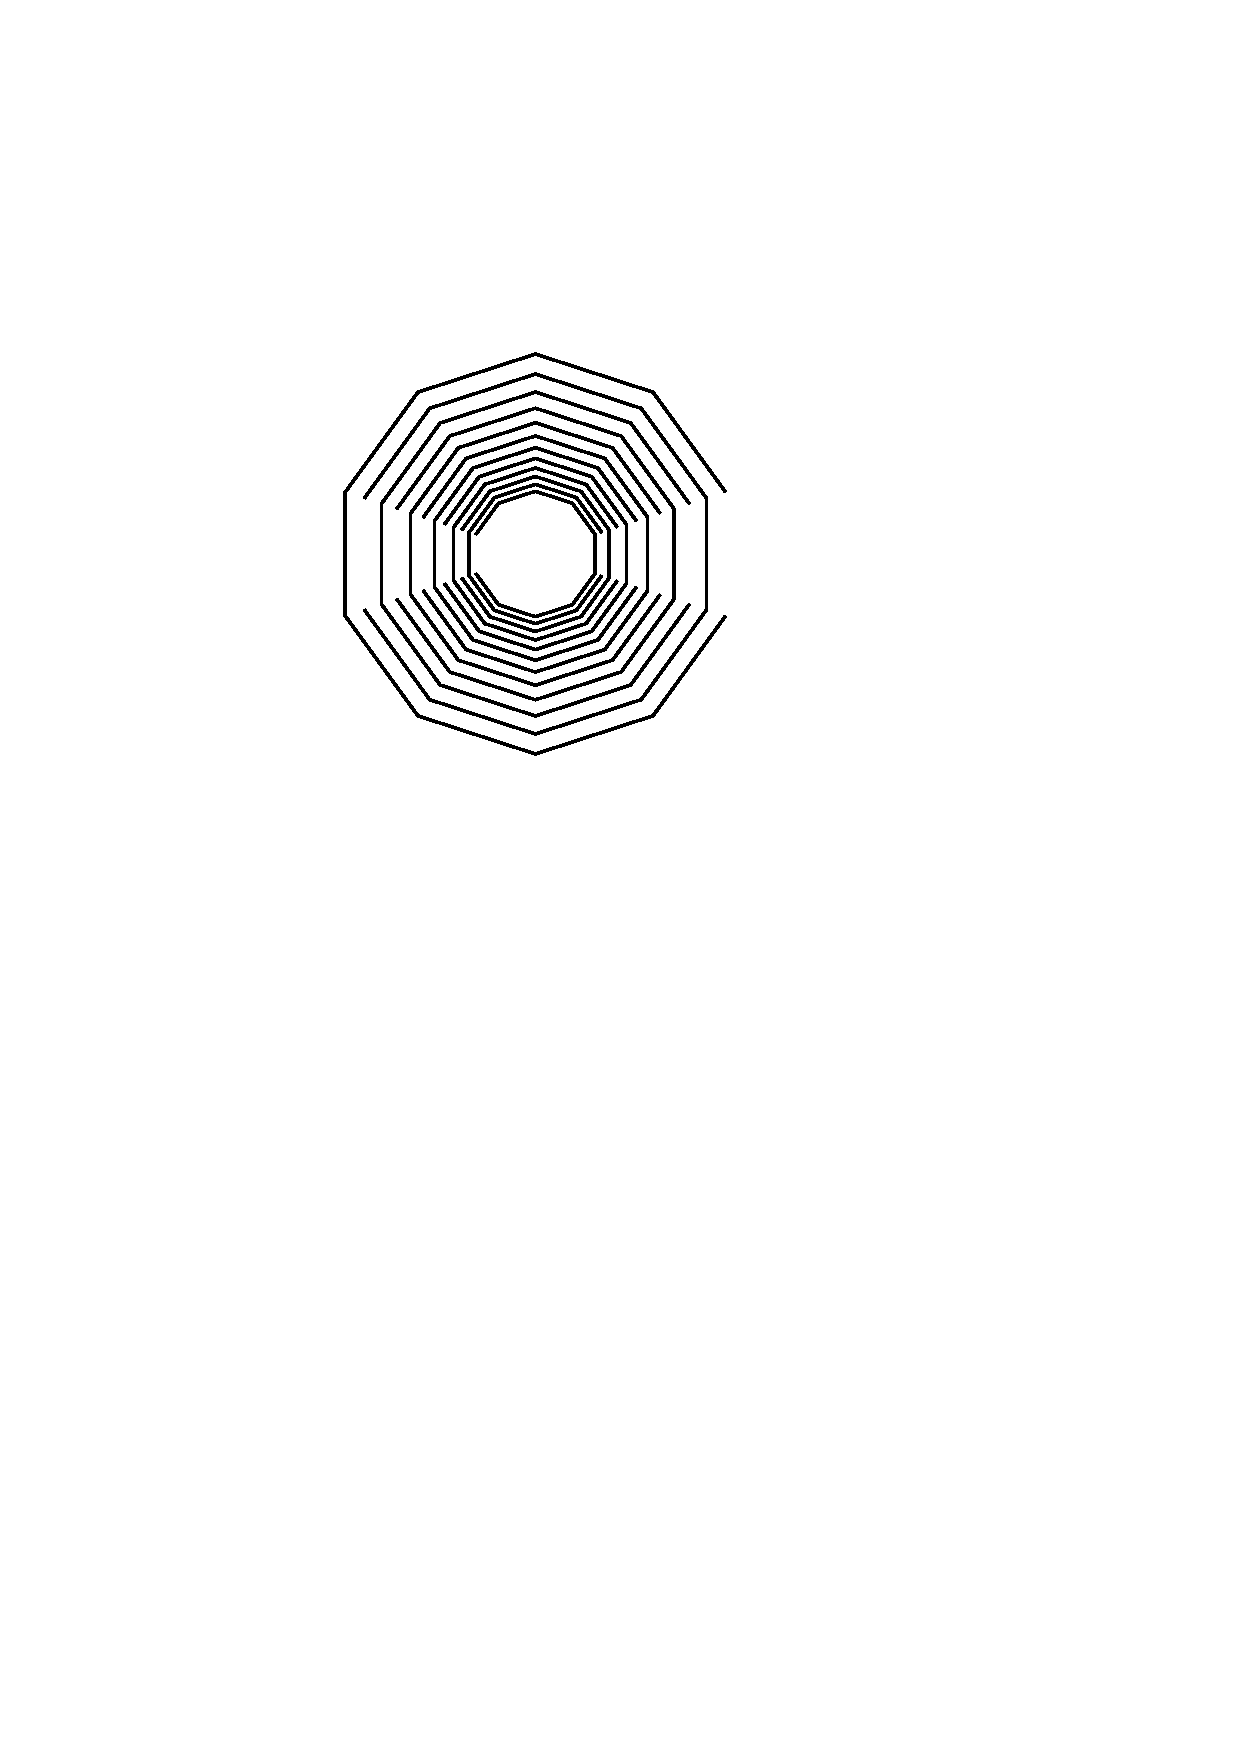
\includegraphics{lower-bound}\end{center}
\caption{An example of two planar objects, $I$ and $I'$ that cannot
be differentiated using $o(1/\qual(I))$ probes.}
\figlabel{lower-bound}
\end{figure}
}

\begin{figure}
\begin{center}\includegraphics{adversary}\end{center}
\caption{An example of two planar objects, $I$ and $I'$ that cannot
be differentiated using $o(1/\qual(I))$ probes.}
\figlabel{lower-bound}
\end{figure}

Assume by way of contradiction that there exists a roundness
classification procedure $\mathcal{P}$ that always accepts $I$ and
always rejects $I'$ using $n< 2\pi(1-\epsilon+\psi)/8\alpha \psi$
probes.  Let $S$ be the set of $n$ probes made by $\mathcal{P}$ in
classifying $I$.  Since $|S|=n<2\pi(1-\epsilon+\psi)/8\alpha\psi$, $S$
contains two probes, $p_1$ and $p_2$, that occur consecutively on
$\bd(I)$, such that the length of $\bd(I)$ between $p_1$ and $p_2$ is
greater than $8\alpha\psi$.  Note that we could place $I'$ with its
recess between $p_1$ and $p_2$, and the results of all the probes made
by $\mathcal{P}$, and therefore the actions of $\mathcal{P}$, would be
the same for $I$ and $I'$.  But this is a contradiction, since we
assumed that $\mathcal{P}$ always correctly classifies both $I$ and
$I'$.

We conclude the proof by making the observation that
$n=2\pi(1-\epsilon+\psi)/8\alpha\psi\in
\Omega(1/\psi)=\Omega(|1/\qual(I)|)=\Omega(|1/\qual(I')|)$. 
\end{proof}

For 3-dimensional objects we require the following lemma.

\begin{lem}\lemlabel{sphere-hide}
Let $S$ be a set of $n^2$ points on the unit sphere.  Then, there
exists a spherical cap $c$ with radius $1/n$ such that $c$ contains no
points of $S$
\end{lem}

\begin{proof}
Consider the convex hull of $S$, which has at most $2n^2-4$ faces.
The plane passing through a face defines a spherical cap, and the
union of these caps cover the entire sphere, a surface area of $4\pi$.
By the pigeonhole principle, some face $f$ must define a cap $c$ with
surface area at least $2\pi/n^2$.  Furthermore, since $f$ is part of
the convex hull, there are no other points of $S$ in this cap.  The
surface area of $c$ obeys the inequality $\sa(c) \le 2\pi r^2$, where
$r$ is the radius of $c$. Thus, we have the inequalities
\[ 2\pi r^2  \ge \sa(c) \ge 2\pi/n^2 \enspace , \]
yielding $r\ge 1/n$.
\end{proof}

\begin{thm}\thmlabel{sphere-lower-bound}
Any roundness classification procedure that is always correct
requires, in the worst case, $\Omega(|1/\qual(I)^2|)$ probes to
classify a object $I$ with center $c_I=\origin$ and satisfying
Assumptions~\ref{ass:mq} and \ref{ass:ss}.
\end{thm}

\begin{proof}
We proceed in almost the same way as in \thmref{lower-bound}.
The object $I$ is a perfect ball with radius $1-\epsilon+\psi$.  The
object $I'$ is similar to $I$, except that it contains a conic recess
of depth $4\psi$ that removes a circle of diameter $8\alpha\psi$ from
the surface of $I$.

Let $S$ be any set of $o(n^2)$ probes directed at $I$.  Then, by
\lemref{sphere-hide}, there exists a spherical cap $c$ on the surface
of $I$ with radius $\omega(\psi)$ such that $c$ contains no point of
$S$.  We use the cap to hide the conic defect of $I'$ so that the
procedure cannot distinguish $I$ and $I'$.
\end{proof}

%%%%%%%%%%%%%%%%%%%%%%%%%%%%%%%%%%%%%%%%%%%%%%%%%%%%%%%%%%%%%%%%%%%%%%%%%%
\section{Conclusions}\seclabel{conclusions}

We have studied the problem of determining whether a manufactured disk
or ball is sufficiently round.  Our model for disks is less
restrictive than that of \cite{msy97,sy95} yet our results are the
same.  Our result for balls is the first result in this area.  We have
also given lower bounds that show that our procedures are optimal in
terms of the number of probes used.

Practitioners may question whether adaptive sampling methods such as
those used in our roundness classification procedures are of wide
spread usefulness, since production facilities are often arranged as
``assembly lines'' in which the each step in the assembly process
should take a fixed, and known, amount of time.  In this case, our
results are still useful, since we can fix the number of probes used
by our procedures.  The bounds on the quality of the object can then
be used to determine whether the object is definitely good, definitely
bad, or unclear.  A conservative production strategy can then simply
reject objects that are bad or unclear.

\section*{Acknowledgement}

The authors would like to thank Silvia~G\"otz for carefully reading
several early revisions of this paper.

\bibliographystyle{plain}
\bibliography{metrology}



\end{document}


